\documentclass[a4paper,14pt]{extarticle}

\usepackage{geometry}
\usepackage[T1]{fontenc}
\usepackage[utf8]{inputenc}
\usepackage[english,russian]{babel}
\usepackage{amsmath}
\usepackage{amsthm}
\usepackage{amssymb}
\usepackage{fancyhdr}
\usepackage{setspace}
\usepackage{graphicx}
\usepackage{lscape}
\usepackage{colortbl}
\usepackage{tikz}
\usepackage{pgf}
\usepackage{subcaption}
\usepackage{listings}
\usepackage{indentfirst}
\usepackage[colorlinks,citecolor=blue,linkcolor=blue,bookmarks=false,hypertexnames=true, urlcolor=blue]{hyperref}
\usepackage{indentfirst}
\usepackage{mathtools}
\usepackage{booktabs}
\usepackage[flushleft]{threeparttable}
\usepackage{tablefootnote}
\usepackage{caption}
\DeclareCaptionLabelSeparator{dash}{ --- }
\captionsetup{
    labelsep=dash
}

\usepackage{chngcntr} % нумерация графиков и таблиц по секциям
\counterwithin{table}{section}
\counterwithin{figure}{section}

\graphicspath{{../graphics/}}%путь к рисункам

\makeatletter
\renewcommand{\@biblabel}[1]{#1.} % Заменяем библиографию с квадратных скобок на точку:
\makeatother

\geometry{left=2.5cm}% левое поле
\geometry{right=1.5cm}% правое поле
\geometry{top=1.5cm}% верхнее поле
\geometry{bottom=1.5cm}% нижнее поле
\renewcommand{\baselinestretch}{1.5} % междустрочный интервал


\newcommand{\bibref}[3]{\hyperlink{#1}{#2 (#3)}} % biblabel, authors, year
\addto\captionsrussian{\def\refname{Список литературы (или источников)}}

\renewcommand{\theenumi}{\arabic{enumi}}% Меняем везде перечисления на цифра.цифра
\renewcommand{\labelenumi}{\arabic{enumi}}% Меняем везде перечисления на цифра.цифра
\renewcommand{\theenumii}{.\arabic{enumii}}% Меняем везде перечисления на цифра.цифра
\renewcommand{\labelenumii}{\arabic{enumi}.\arabic{enumii}.}% Меняем везде перечисления на цифра.цифра
\renewcommand{\theenumiii}{.\arabic{enumiii}}% Меняем везде перечисления на цифра.цифра
\renewcommand{\labelenumiii}{\arabic{enumi}.\arabic{enumii}.\arabic{enumiii}.}% Меняем везде перечисления на цифра.цифра

\begin{document}
\begin{titlepage}
\newpage

{\setstretch{1.0}
\begin{center}
Federal State Autonomous Educational Institution for Higher Education
National Research University Higher School of Economics
\\
\bigskip
Faculty of Computer Science \\
Applied Mathematics and Information Science \\
\end{center}
}

\vspace{8em}

\begin{center}
{\Large BACHELOR'S THESIS}\\
\textsc{\textbf{
Research project
\linebreak
"Your Theme"}}
\end{center}

\vspace{4em}

{\setstretch{1.0}
\hfill\parbox{16cm}{
\hspace*{5cm}\hspace*{-5cm}Prepared by the student of group 171, 4th year of study,\\
Gelvan Kirill Pavlovich\\

\hspace*{5cm}\hspace*{-5cm}Supervisor:\\
Senior Research Fellow, Nadezhda Chirkova
\\

\hspace*{5cm}\hspace*{-5cm}Curator:\\
...\\

\hspace*{5cm}\hspace*{-5cm}Consultant:\\
...\\
}
}

\vspace{\fill}

\begin{center}
Moscow 2021
\end{center}

\end{titlepage}
% это титульный лист
\newpage
\setcounter{page}{2}

{
    \hypersetup{linkcolor=black}
    \tableofcontents
}

% \newpage
% \section{Примеры} 
\subsection{Ссылки на статьи}

Можно ссылаться на статью вот так:  \bibref{chirkova18}{Chirkova et al.}{2017}.

\subsection{График}

График \ref{fig:by_epochs} достаточно бессмысленный без контекста.

\begin{figure}[h!]
	\centering
	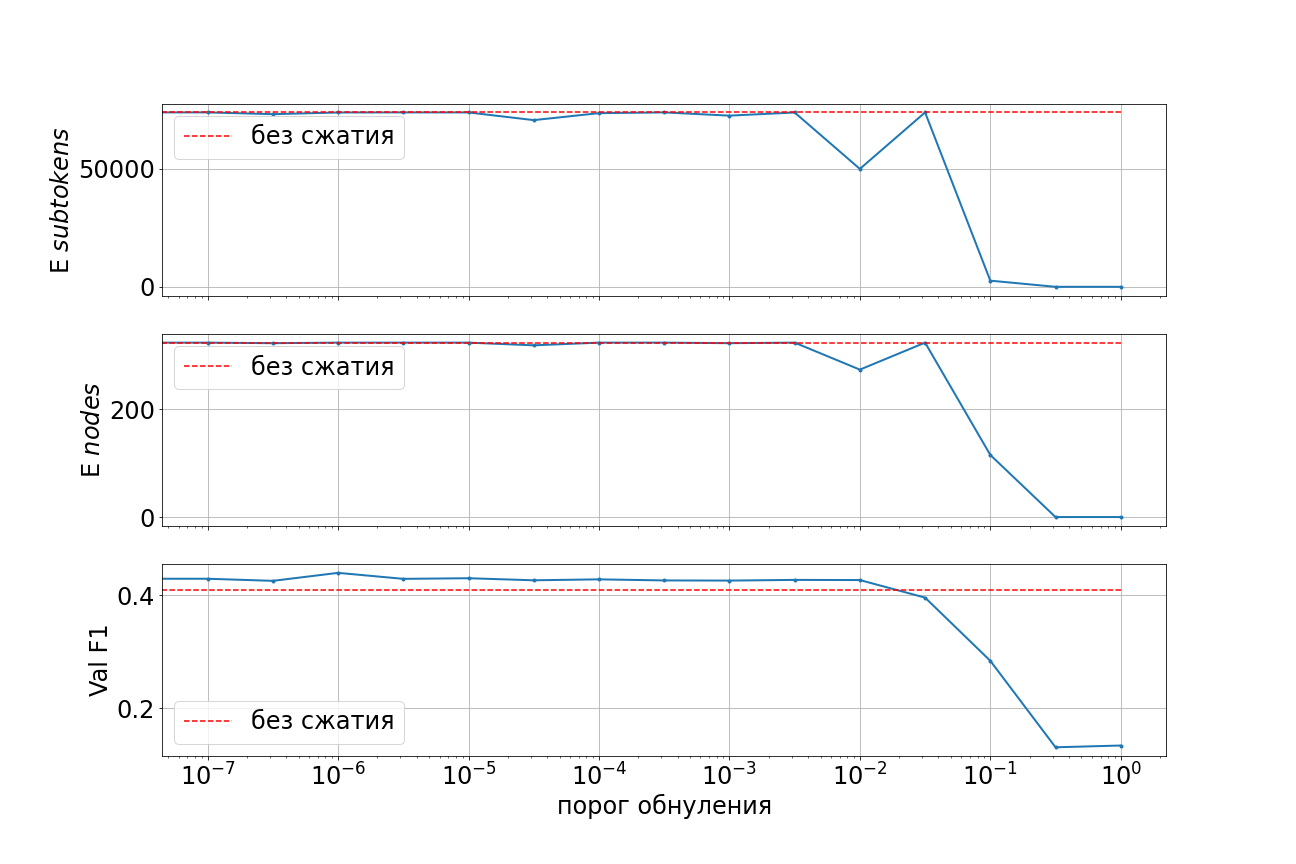
\includegraphics[width=1\textwidth]{example.png}
	\caption{Пример графика}
	\label{fig:by_epochs}
\end{figure}


\subsection{Таблица}

\begin{table}[htbp]
	\caption{Пример таблички}
	\label{table:long_epochs}
	\footnotesize
	\centering
	\begin{tabular}{lrrrrrrrr}
		\toprule
		& \multicolumn{3}{c}{$\mathsf{Val}$} &
		\multicolumn{3}{c}{$\mathsf{Test}$} \\
		\cmidrule(lr){2-4} \cmidrule(l){5-7} 
		{} &  $\mathsf{Prec}$ &  $\mathsf{Rec}$ &  $\mathsf{F1}$ &  $\mathsf{Prec}$ &  $\mathsf{Rec}$ &  $\mathsf{F1}$  &  $\mathsf{nodes}$ & $\mathsf{subtokens}$\\
		\midrule
		запуск 1    &    0.4894 &   0.3775 &  0.4263 &     0.4824 &    0.3683 &   0.4177 & 10029 & 179\\
		запуск 2    &    0.4887 &   0.3739 &  0.4237 &     0.4891 &    0.3724 &   0.4228 & 10039 & 177\\
		запуск 3    &    0.4820 &   0.3751 &  0.4219 &     0.4838 &    0.3677 &   0.4178 & 10037&	180\\
		\midrule
		\bf{среднее} &    \bf{0.4867} &   \bf{0.3755} &  \bf{0.4239} &    \bf{ 0.4851} &    \bf{0.3695} &   \bf{0.4195} \\
		\bf{дисперсия}  &    0.0041 &   0.0019 &  0.0022 &     0.0036 &    0.0025 &   0.0029 \\
		\bottomrule
	\end{tabular}
\end{table}

\newpage
\section{Постановка задачи}

Данная курсовая работа направлена на разработку распределенной асинхронной системы обработки real-time финансовых данных. Задача работы заключается в создании программного продукта, способного обрабатывать большие объемы данных в режиме реального времени, с целью предоставления пользователю актуальной информации о финансовых инструментах.

Для достижения поставленной цели необходимо решить следующие задачи:
\begin{itemize}
    \item  Разработать архитектуру системы, которая бы обеспечивала высокую производительность и масштабируемость программного продукта;
    \item  Реализовать механизмы асинхронной обработки данных, позволяющие обрабатывать большие объемы информации в режиме реального времени;
    \item  Разработать механизмы распределенной обработки данных, позволяющие обрабатывать данные на нескольких серверах;
    \item  Реализовать механизмы мониторинга и управления системой для обеспечения ее стабильной работы;
    \item  Разработать механизмы взаимодействия с пользователем, позволяющие предоставлять актуальную информацию о финансовых инструментах в режиме реального времени.
\end{itemize}

Итоговое приложение, созданное в рамках данной курсовой работы, должно включать в себя следующие компоненты:

\begin{itemize}
    \item Модуль сбора данных: этот модуль должен быть способен собирать данные из различных источников, таких как торговые площадки, криптовалютные биржи и т.д.
    \item Модуль обработки данных: этот модуль должен обрабатывать данные, полученные от модуля сбора данных.
    \item Модуль представления данных: этот модуль должен предоставлять пользователю актуальную информацию о финансовых инструментах в режиме реального времени.
          Для этого могут использоваться различные методы представления данных, такие как графики, диаграммы, таблицы и т.д.
    \item Модуль управления системой: этот модуль должен обеспечивать стабильную работу системы, включая мониторинг производительности, управление ресурсами и т.д.
\end{itemize}

В результате выполнения данной курсовой работы будет создан программный продукт, который сможет обрабатывать большие объемы данных в режиме реального времени, обеспечивая пользователю актуальную информацию о финансовых инструментах.


\newpage
\section{Обоснование актуальности и новизны}
Актуальность нашего проекта обусловлена несколькими ключевыми факторами:

\begin{itemize}
    \item Отсутствие качественных альтернатив: После ухода известных платформ на рынке осталось немного приложений, которые бы предлагали действительно качественный и современный сервис знакомств. Пользователи ищут новые способы для поиска партнера, которые не были бы ограничены лишь визуальной оценкой.
    \item Изменение предпочтений пользователей: Современные пользователи все больше ценят содержание и смысл в общении. Они стремятся находить партнеров, с которыми у них есть общие интересы и взгляды на жизнь, а не просто симпатичную внешность. Традиционная система свайпов не отвечает этим требованиям и часто приводит к разочарованию и потере интереса к приложениям для знакомств.
    \item Социальная изоляция: В условиях пандемии и социальной изоляции значимость онлайн-знакомств возросла многократно. Люди ищут возможности для установления новых социальных связей и хотят, чтобы эти связи основывались на чем-то большем, чем просто фотографии.
\end{itemize}



Наш проект предлагает новый подход к онлайн-знакомствам, который соответствует современным требованиям и ожиданиям пользователей:

\begin{itemize}
    \item Фокус на содержании: Вместо того чтобы полагаться исключительно на фотографии, наше приложение предоставляет возможность выделяться с помощью интересных и цепляющих предложений для разговора. Это способствует созданию более глубоких и осмысленных взаимодействий между пользователями.
    \item Интерактивность и многообразие: Мы предлагаем интеграцию голосовых промптов, что добавляет новое измерение в процесс знакомства и позволяет пользователям выразить свою личность более полно.
\end{itemize}


Новизна нашего проекта заключается в сочетании интерактивных элементов, фокусе на содержании и удобстве использования, что отличает его от существующих решений на рынке. Мы стремимся создать платформу, которая не только удовлетворяет потребности пользователей, но и предлагает новые, эффективные способы для установления значимых отношений.






\newpage
\section{Обзор существующих решений}

Существует несколько систем для обработки финансовых данных в реальном времени.
Одной из таких систем является Bloomberg Terminal. Это финансовая платформа,
которая предоставляет доступ к рыночным данным, новостям, аналитическим
инструментам и торговым системам. Bloomberg Terminal является популярным
инструментом для трейдеров и инвесторов, так как позволяет получать актуальную
информацию о финансовых рынках в режиме реального времени.

Еще одной системой для обработки финансовых данных в реальном времени является
Thomson Reuters Eikon. Это платформа, которая предоставляет доступ к рыночным
данным, новостям, аналитическим инструментам и торговым системам. Thomson
Reuters Eikon также позволяет получать актуальную информацию о финансовых рынках
в режиме реального времени.

Кроме того, существуют системы, которые предоставляют доступ к финансовым
данным в режиме реального времени через API. Например, Alpha Vantage API
предоставляет доступ к актуальным данным о финансовых рынках, таким как
котировки, графики и новости. Alpha Vantage API имеет бесплатный план, который
позволяет получать до 500 запросов в день, а также платные планы с более
высокими лимитами.

Каждая из этих систем имеет свои преимущества и недостатки, и выбор конкретной
системы зависит от требований проекта и доступных ресурсов. В разработке
распределенной системы для обработки финансовых данных в реальном времени
необходимо учитывать не только функциональные требования, но и требования по
производительности, масштабируемости и отказоустойчивости.

% \newpage
% \section{Выбор инструментальных средств разработки}

В процессе разработки распределенной системы для обработки финансовых данных в реальном времени я использовал ряд инструментальных средств.

Основным языком программирования, который я использовал, был Java 17. Это популярный язык программирования, который позволяет разрабатывать высокопроизводительные и масштабируемые приложения.

Для разработки микросервисов я использовал Spring Boot и Spring Cloud OpenFeign. Spring Boot - это фреймворк для разработки микросервисов на языке Java, который позволяет ускорить процесс разработки и упростить конфигурацию приложения. Spring Cloud OpenFeign - это библиотека, которая позволяет создавать клиенты для микросервисов на основе аннотаций.

Для обмена сообщениями между микросервисами я использовал Apache Kafka. Это распределенная платформа для потоковой обработки данных, которая позволяет обрабатывать потоки данных в реальном времени.

Для контейнеризации приложения я использовал Docker и docker-compose. Docker - это платформа для создания, развертывания и управления контейнерами, которая позволяет упростить процесс разработки и развертывания приложения. Docker-compose - это инструмент, который позволяет запускать несколько контейнеров вместе и управлять ими.

Для мониторинга и управления приложением я использовал Prometheus и Grafana. Prometheus - это система мониторинга, которая позволяет собирать метрики приложения и анализировать их. Grafana - это инструмент визуализации данных, который позволяет отображать метрики приложения в виде графиков и диаграмм.

Для хранения данных я использовал базу данных PostgreSQL и Spring Data JPA. PostgreSQL - это реляционная база данных, которая позволяет хранить и управлять данными. Spring Data JPA - это библиотека, которая позволяет упростить работу с базой данных и ускорить процесс разработки.

Каждый из этих инструментов был выбран с учетом требований проекта и доступных ресурсов. Вместе они позволили разработать высокопроизводительную и масштабируемую систему для обработки финансовых данных в реальном времени.

% \newpage
% \section{Проектирование реализации}


\begin{figure}[h]
    \centering
    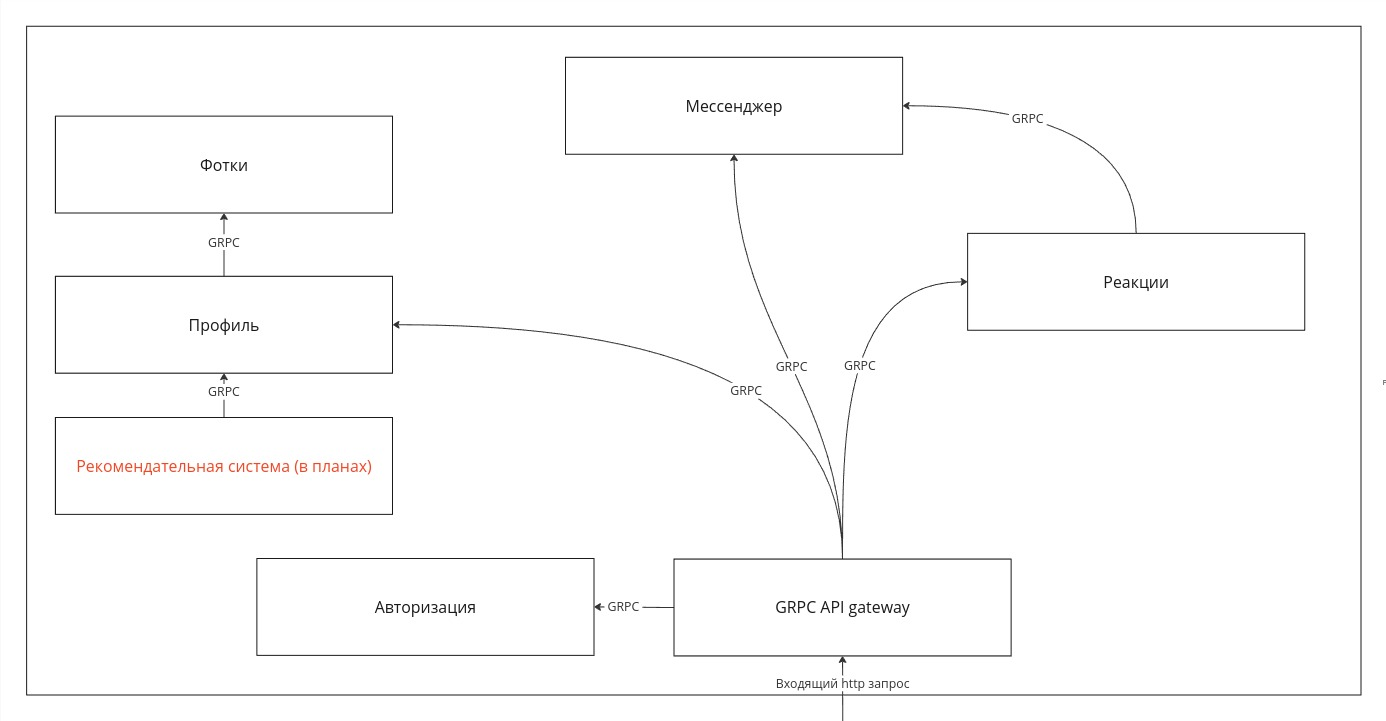
\includegraphics[width=1\columnwidth ]{glimpse - Схема межсервисного взаимодействия.jpg}
    \caption{C2 модель архитектуры}
\end{figure}

В данном разделе рассмотрим проектирование реализации нашего приложения для знакомств, основанного на микросервисной архитектуре. Схема межсервисного взаимодействия представлена на рисунке и описывает, как различные компоненты приложения взаимодействуют друг с другом посредством \textbf{gRPC}.

\textbf{Основные компоненты системы:}

\begin{itemize}
    \item \textbf{GRPC API Gateway:} Этот компонент служит центральной точкой входа для всех HTTP-запросов, поступающих в систему. API Gateway принимает запросы от клиентов и маршрутизирует их к соответствующим микросервисам, используя gRPC. Это обеспечивает единый интерфейс для внешних взаимодействий и упрощает управление трафиком.
    
    \item \textbf{Авторизация:} Микросервис, отвечающий за аутентификацию и регистрацию пользователей. Он обрабатывает запросы на вход в систему, проверяет учетные данные пользователей и выдает токены доступа, которые используются для последующих запросов через API Gateway.
    
    \item \textbf{Профиль:} Микросервис, управляющий профилями пользователей. Он обрабатывает запросы на создание, редактирование и удаление профилей, а также хранит и предоставляет данные профилей другим микросервисам по gRPC.
    
    \item \textbf{Фотки:} Этот микросервис отвечает за загрузку и хранение фотографий пользователей. Он взаимодействует с микросервисом профилей для привязки фотографий к соответствующим профилям пользователей.
    
    \item \textbf{Мессенджер:} Микросервис для обмена сообщениями между пользователями. Использует ScyllaDB для хранения сообщений и обеспечивает возможность отправки и получения текстовых и голосовых сообщений.
    
    \item \textbf{Реакции:} Микросервис, который управляет реакциями пользователей на профили других пользователей. Он обрабатывает лайки, дизлайки и другие виды реакций, а также предоставляет данные о реакциях другим компонентам системы.
    
    \item \textbf{Рекомендательная система (в планах):} Будет разработана для предоставления пользователям персонализированных рекомендаций на основе их профилей и поведения в приложении. Этот микросервис будет взаимодействовать с профилем и реакциями для получения необходимых данных.
\end{itemize}

\textbf{Межсервисное взаимодействие:}

Все микросервисы взаимодействуют друг с другом с помощью gRPC, что обеспечивает высокую производительность и низкую задержку при обмене данными. Основные потоки данных и взаимодействия между микросервисами включают:

\begin{itemize}
    \item API Gateway принимает входящие HTTP-запросы от клиентов и маршрутизирует их к соответствующим микросервисам через gRPC.
    \item Микросервис Авторизации взаимодействует с API Gateway для аутентификации пользователей и выдачи токенов доступа.
    \item Микросервис Профилей взаимодействует с Фотками для управления фотографиями пользователей и с Реакциями для обработки реакций на профили.
    \item Мессенджер взаимодействует с Реакциями и Профилями для обеспечения контекста сообщений и управления диалогами.
    \item В перспективе, Рекомендательная система будет интегрирована с Профилями и Реакциями для предоставления персонализированных рекомендаций пользователям.
\end{itemize}

Такое проектирование обеспечивает модульность, масштабируемость и гибкость системы, что позволяет легко добавлять новые функции и улучшать существующие компоненты без значительных изменений в архитектуре приложения.


% \clearpage
% \section{Описание программной системы}

В рамках курсовой работы я разработал программное обеспечение для
обработки real-time финансовых данных. Система работает на основе
распределенной асинхронной архитектуры и состоит из нескольких сервисов, каждый
из которых выполняет свою функцию.

Один из основных сервисов - это сервис producer-ms, который получает данные из
API провайдера финансовых данных каждые n секунд. В этом случае я использовал
coin market cap в качестве провайдера. Эти данные отправляются в шину kafka, где
перехватываются фильтром.

Сервис filter-ms отвечает за фильтрацию данных и приведение их в один тип
сущности.
К примеру, для криптовалют приводится к следующему типу:

\begin{table}[h!]
    \caption{Тип сущности в базе данных для криптовалют}
    \begin{center}
        \begin{tabular}{|l|l|p{9cm}|}
            \hline
            symbol              & string    & обозначает символ для криптовалюты (например BTC для биткоина) \\
            \hline
            vendor              & bigint    & внешний ключ для вендора                                       \\
            \hline
            observed\_at        & timestamp & время, в котором эти данные были зафиксированы                 \\
            \hline
            max\_supply         & bigint    & максимальное объем криптовалюты                                \\
            \hline
            circulating\_supply & bigint    & циркулирующий объем криптовалюты                               \\
            \hline
            total\_supply       & bigint    & общий объем криптовалюты                                       \\
            \hline
            price\_usd          & double    & цена криптовалюты в долларах                                   \\
            \hline
            volume\_24h         & double    & процент капитализации рынка                                    \\
            \hline
            market\_cap         & double    & капитализация рынка                                            \\
            \hline
        \end{tabular}
    \end{center}
\end{table}

В этом случае я работал с криптовалютами, но при расширении система может
работать и с фиатом и ценными бумагами. После фильтрации данные
отправляются в шину kafka, где их перехватывает загрузчик.

Сервис loader-ms отвечает за загрузку сущностей в базу данных PostgreSQL. Здесь
я использую мощные возможности PostgreSQL для хранения и обработки больших
объемов данных. В результате получился быстрый и надежный доступ к финансовым
данным.

Система также включает в себя сервис report-builder, который позволяет
пользователям получать доступ к обработанным данным. С помощью report-builder
пользователи могут получать различные отчеты и аналитические данные, которые
могут быть использованы для принятия финансовых решений.

\begin{figure}[h]
    \centering
    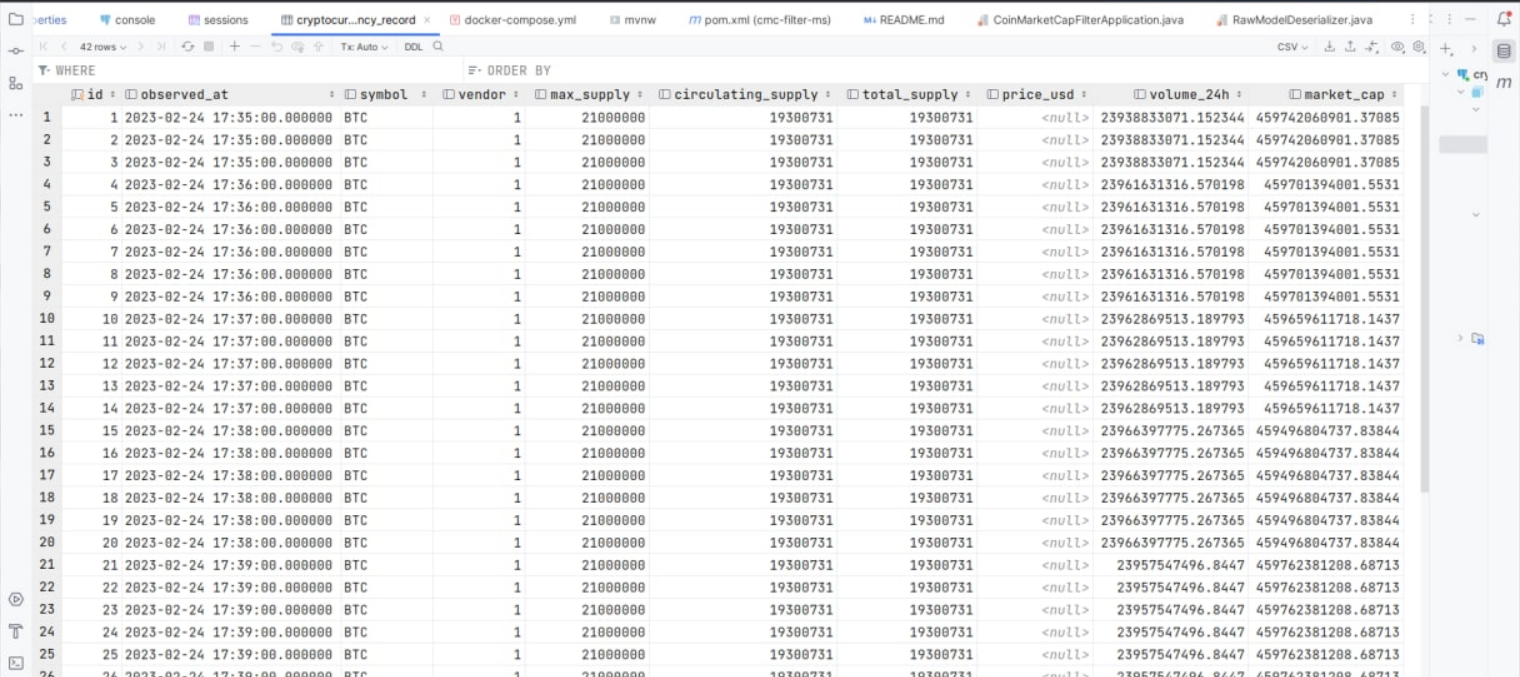
\includegraphics[width=1\columnwidth]{databasescreen.png}
    \caption{Изображение с содержанием базы данных }
\end{figure}

Также благодаря сбору метрик был реализован простой UI с помощью Prometheus и Grafana
для отображения системной информации о загруженности системы, а также графики
стоимости криптовалют за наблюдаемый промежуток.

\begin{landscape}
    \begin{figure}[!h]
        \centering
        % 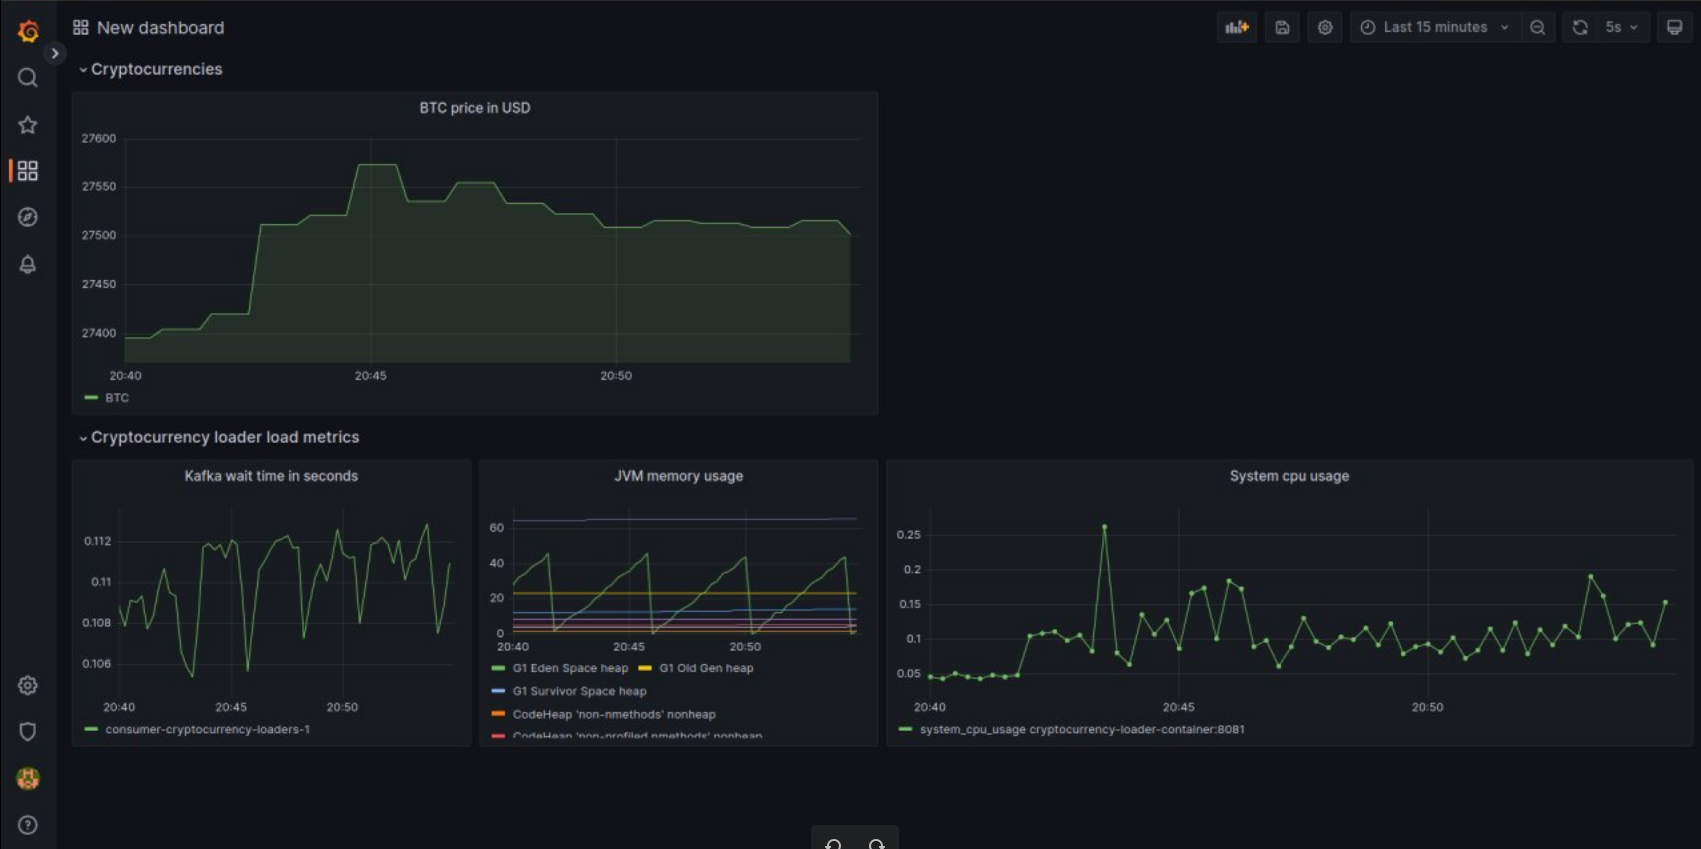
\includegraphics[width=1\columnwidth]{grafanascreen.png}
        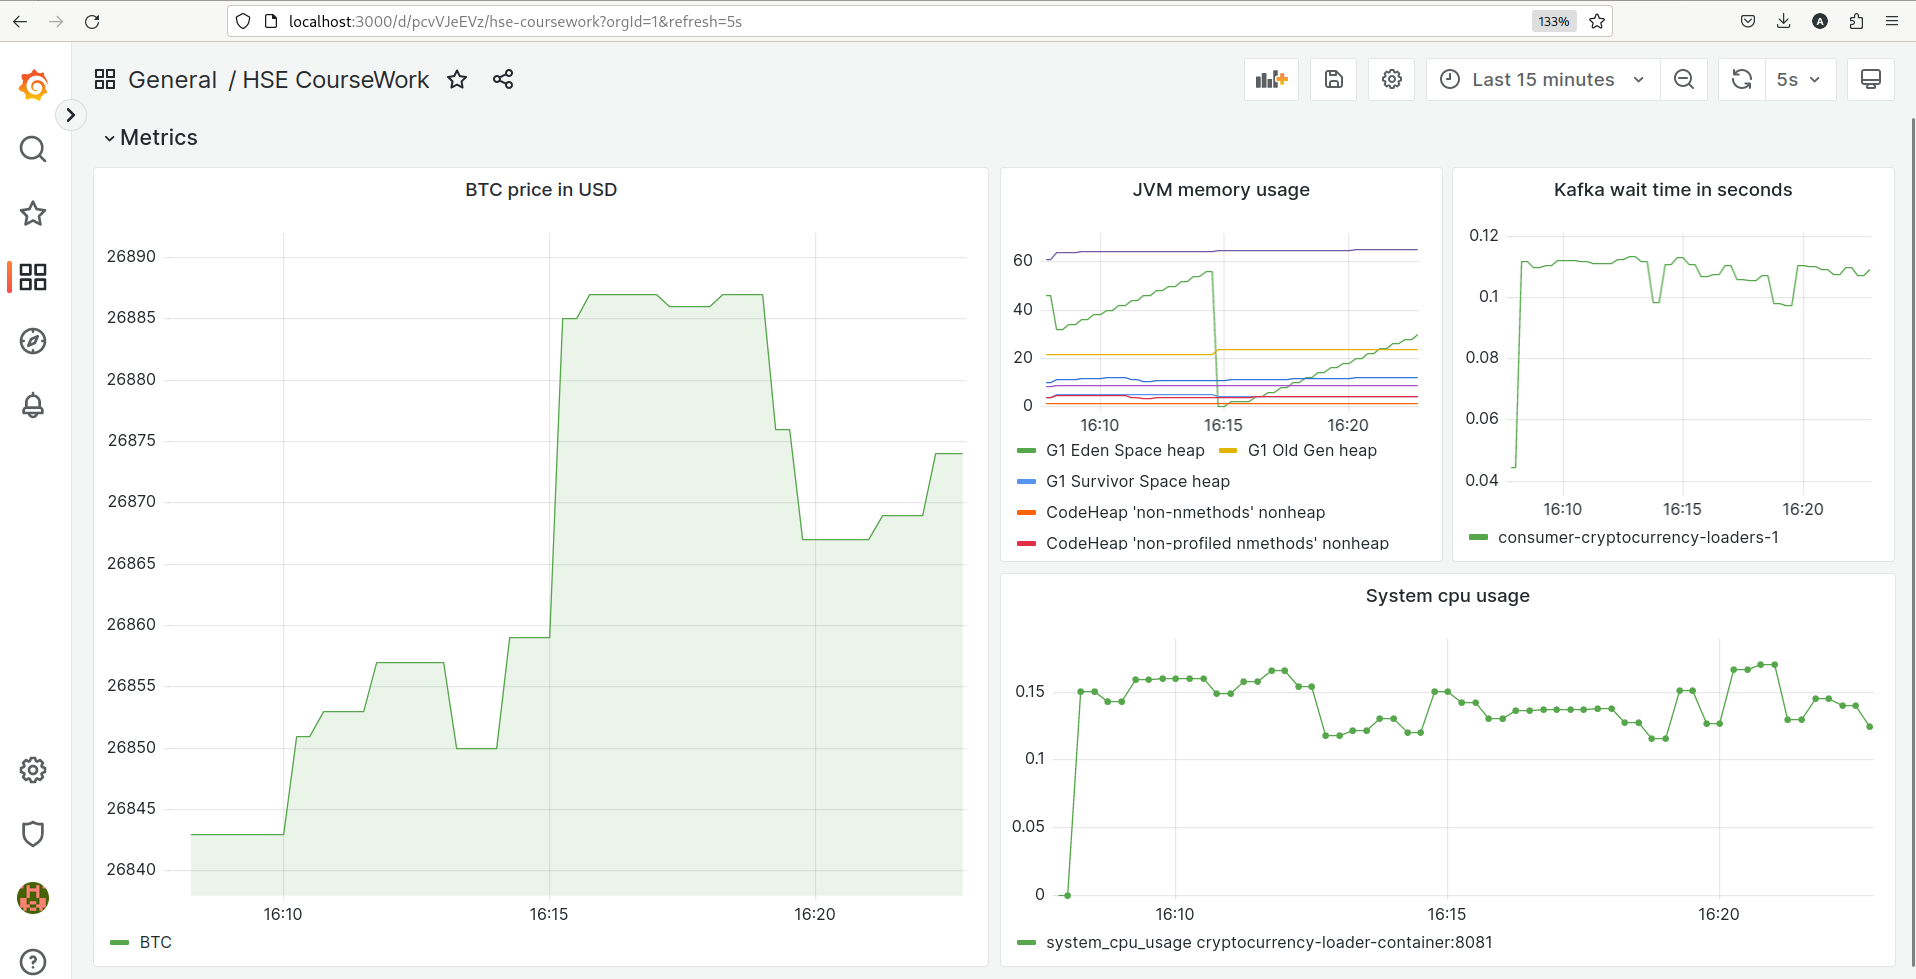
\includegraphics[height=0.8\textheight]{grafanav2.png}
        \caption{Изображение дашборда Grafana с графиком цены биткоина и системными метриками загруженности.}
        \label{grafana}
    \end{figure}
\end{landscape}

В целом система представляет собой мощный инструмент для обработки
real-time финансовых данных. Я использовал современные технологии и подходы,
чтобы обеспечить быстрый и надежный доступ к данным для наших пользователей. В
результате получилась высокоэффективная система, которая может быть
использована в различных областях финансовой деятельности.


% \clearpage
% \section{Методика и результаты тестирования}

Для тестирования программной системы я использовал различные методы и инструменты. Я провел ручное тестирование, а также интеграционное тестирование с помощью Spring Boot Test и testcontainers, а также unit тестирование с помощью JUnit5 и Mockito.

Ручное тестирование позволило проверить правильность работы системы и выявить возможные ошибки и проблемы. Также было произведено тестирование на различных этапах разработки, начиная с тестирования каждого отдельного сервиса и заканчивая тестированием всей системы в целом.

Интеграционное тестирование с помощью Spring Boot Test и testcontainers позволило проверить работу системы в целом, а также проверить работу каждого сервиса внутри системы. Было использовано testcontainers для запуска контейнеров с базой данных PostgreSQL и кафкой, что позволило проводить тестирование в реальных условиях.

Unit тестирование с помощью JUnit5 и Mockito позволило проверить правильность работы каждого отдельного компонента системы. Было использовано Mockito для подмены зависимостей и создания тестовых сценариев.

В целом, методика тестирования была основана на принципах современной методологии тестирования, которая включает
в себя ряд принципов и методов,
которые помогают создавать качественные, надежные и эффективные программные
продукты. Вот некоторые из них:

\begin{itemize}
    \item Автоматизированное тестирование. Автоматизированные тесты позволяют повторять тестовые сценарии быстро и точно, что позволяет выявлять проблемы и ошибки на ранних стадиях разработки.
    \item Интеграционное тестирование. Интеграционное тестирование позволяет проверять, как различные компоненты программного продукта взаимодействуют друг с другом, что позволяет выявлять проблемы и ошибки на ранних стадиях разработки.
    \item Unit-тестирование. Unit-тестирование позволяет проверять отдельные модули кода на корректность и соответствие требованиям, что позволяет выявлять проблемы и ошибки на ранних стадиях разработки.
    \item Контейнеризация для интеграционного тестирования. Контейнеризация позволяет создавать изолированные среды для интеграционного тестирования, что помогает избежать проблем с зависимостями и конфигурацией.
    \item Мокирование зависимостей для unit-тестирования. Мокирование зависимостей позволяет создавать тестовые сценарии для отдельных модулей кода, не зависящих от других модулей, что позволяет выявлять проблемы и ошибки на ранних стадиях разработки.
\end{itemize}

Эти принципы и методы помогают создавать качественные программные продукты и
обеспечивать их надежность и эффективность.

После проведения тестирования получились положительные результаты. Система работает стабильно и быстро обрабатывает финансовые данные в реальном времени. Были выявлены и устранены некоторые ошибки и проблемы в процессе тестирования, что позволило создать надежную и эффективную систему для обработки финансовых данных. В результате работы получилась высокоэффективная система, которая может быть использована в различных областях финансовой деятельности.

% \newpage
% \section{Пути возможного развития}

На основе результатов проведенного нагрузочного тестирования и анализа текущих возможностей системы, были выявлены несколько направлений для дальнейшего развития и улучшения нашего приложения для знакомств.

\textbf{Улучшение архитектуры мессенджера:}
Результаты нагрузочного тестирования показали, что архитектура мессенджера требует оптимизации для обеспечения стабильной работы под высокими нагрузками. Для этого планируется:
\begin{itemize}
    \item Оптимизировать текущую архитектуру мессенджера для повышения производительности.
    \item Внедрить механизмы горизонтального масштабирования для обработки большого количества одновременных пользователей.
    \item Улучшить механизмы кэширования и обработки сообщений для снижения задержек.
\end{itemize}

\textbf{Расширение функциональности мессенджера:}
Для повышения удобства и расширения возможностей взаимодействия между пользователями, необходимо добавить следующие функции:
\begin{itemize}
    \item Возможность отправки голосовых сообщений, что позволит пользователям выражать свои эмоции и мысли более полно.
    \item Поддержка отправки сообщений с фотографиями и файлами для разнообразия общения и обмена информацией.
\end{itemize}

\textbf{Разработка рекомендательной системы:}
Для улучшения качества знакомств и повышения удовлетворенности пользователей необходимо внедрить продвинутую рекомендательную систему. Эта система будет:
\begin{itemize}
    \item Основываться на психологическом портрете пользователя, учитывая его интересы, предпочтения и поведение в приложении.
    \item Использовать машинное обучение для персонализации рекомендаций и повышения их точности.
    \item Интегрироваться с текущими микросервисами для обеспечения бесшовного взаимодействия и актуальности данных.
\end{itemize}

\textbf{Улучшение CI/CD процессов:}
Для обеспечения быстрой и надежной выкладки новых функциональностей из тестовой среды в продуктовую необходимо улучшить процессы CI/CD. В планах:
\begin{itemize}
    \item Автоматизировать процессы тестирования и развертывания новых версий микросервисов.
    \item Оптимизировать pipeline для сокращения времени развертывания и повышения стабильности релизов.
\end{itemize}

Реализация этих улучшений позволит нам создать более стабильное, функциональное и удобное приложение, которое будет отвечать потребностям пользователей и соответствовать современным стандартам качества.



% \newpage
% \section{Документация к программе}

Документация к программе --- это один из самых важных аспектов в разработке
программного обеспечения. В рамках курсовой работы на тему ``Разработка
распределенной асинхронной системы обработки real-time финансовых данных'' было
уделено большое внимание документированию API приложения. Для этого было
использовано OpenAPI.

OpenAPI --- это язык описания RESTful API, который позволяет разработчикам
создавать и документировать API для своих приложений. Он позволяет определить
все доступные ресурсы, методы, параметры и схемы данных, которые используются в
приложении. OpenAPI является полезным инструментом для разработчиков, поскольку
он помогает им легко создавать и поддерживать API, а также упрощает процесс
интеграции с другими приложениями.

Для документирования API приложения было использовано Swagger UI ---
инструмент, который позволяет визуально отображать и тестировать API. На рисунке \ref{swager}
вы можете увидеть пример того, как выглядит документация нашего API в Swagger UI.
Здесь можно увидеть все доступные ресурсы, методы и параметры, а также выполнить
тестирование каждого метода.

\begin{figure}[h]
    \centering
    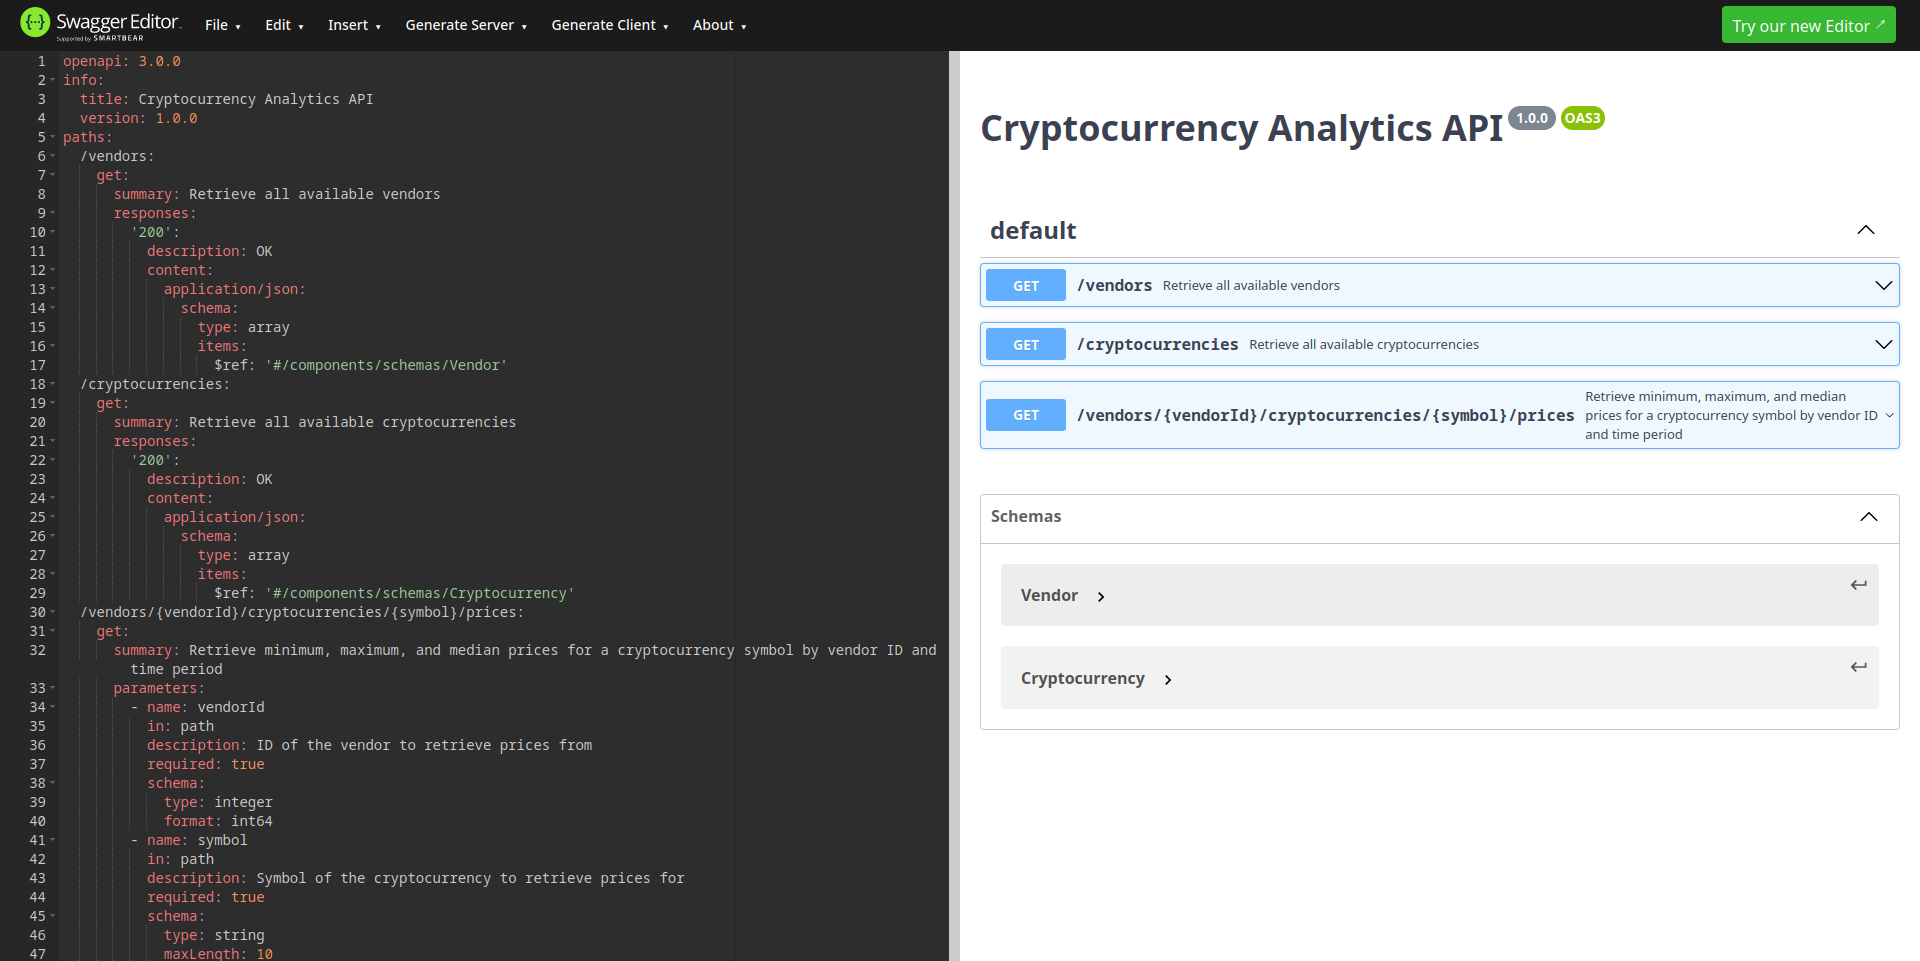
\includegraphics[width=1\linewidth]{swagerscreen.png}
    \caption{Изображение Swagger Editor с документацией к API приложения}
    \label{swager}
\end{figure}

OpenAPI документация помогает разработчикам легко создавать и поддерживать API,
а также упрощает процесс интеграции с другими приложениями. Она также
обеспечивает единый стандарт для описания API, что позволяет разработчикам легко
понимать и использовать API других приложений.

Приложение также может работать как автономное приложение, если
подключиться к Grafana и смотреть цены на криптовалюту используя
разработанный дашборд (см. Рис \ref{grafana}).
Grafana --- это инструмент для визуализации данных,
который позволяет отображать данные в режиме реального времени. Дашборд
позволяет отслеживать цены на криптовалюту в режиме реального времени и
анализировать изменения цен с помощью графиков и диаграмм.

Таким образом, в рамках разработки распределенной асинхронной системы
обработки real-time финансовых данных было уделено большое внимание
документированию API приложения. Использование OpenAPI позволило
легко создавать и поддерживать API, а также упрощал процесс интеграции с другими
приложениями. Итоговое приложение также может работать как автономное приложение,
если подключиться к Grafana и использовать разработанный дашборд для
отслеживания цен на криптовалюту в режиме реального времени.

% \newpage
% \section{Ссылка на хранилище исходного кода}

Весь исходный код программного обеспечения находится в организации на \href{
      https://github.com/orgs/soulmate-dating/repositories}{Github}.

Перечислю и опишу используемые репозитории:
\begin{enumerate}
      \item Репозиторий \href{https://github.com/soulmate-dating/glimpse-compose}{glimpse-compose}
            хранит файл docker-compose для запуска всего приложения, а также файлы
            описывающие манифесты для разворачивания сервисов в Kubernetes.

      \item Репозиторий \href{https://github.com/soulmate-dating/reactions}{reactions}
            хранит исходный код сервиса для реакций пользователей на других пользователей.

      \item Репозиторий \href{https://github.com/soulmate-dating/messenger}{messenger}
            хранит исходный код сервиса для обмена сообщениями между пользователями.

      \item Репозиторий \href{https://github.com/soulmate-dating/profiles}
            {profiles}
            хранит исходный код сервиса для работы с профилями пользователей.

      \item Репозиторий \href{https://github.com/soulmate-dating/gandalf-gateway}{gandal-gateway}
            хранит исходный код сервиса для маршрутизации запросов к другим сервисам через GRPC.

      \item Репозиторий \href{https://github.com/soulmate-dating/auth}{auth}
            хранит исходный код сервиса для аутентификации и регистрации пользователей.

      \item Репозиторий \href{https://github.com/soulmate-dating/media}{media}
            хранит исходный код сервиса для работы с медиа-файлами (фотографии, голосовые сообщения).

\end{enumerate}

% \newpage
% \section{Личный вклад в развитие проекта}

В рамках данной курсовой работы я занимался разработкой двух ключевых микросервисов: \textbf{messenger} (для общения пользователей) и \textbf{reactions} (для обработки реакций пользователей на предложения для общения других пользователей).

\textbf{Messenger:} 
Для реализации сервиса messenger я использовал Java 21 и Spring Boot 3 с подключением к базе данных ScyllaDB. Я спроектировал таблицу для хранения сообщений с учетом всех ограничений ScyllaDB. Структура таблицы выглядит следующим образом:

\begin{figure}[h]
    \begin{verbatim}
    create table if not exists messages
    (
        companions_composite_key text,
        id                       timeuuid,
        sender_id                uuid,
        recipient_id             uuid,
        date                     timestamp,
        content                  text,
        tag_name                 text,
        tag_external_id          uuid,
        PRIMARY KEY (companions_composite_key, id)
    ) with clustering order by (id desc);
    \end{verbatim}
    \caption{Описание таблицы с сообщениями в базе данных}
\end{figure}

В данной таблице:
\begin{itemize}
    \item \textbf{companions\_composite\_key} используется как разделяющий ключ для обеспечения равномерного распределения данных по узлам кластера.
    \item \textbf{id} (timeuuid) используется как кластеризующий ключ для упорядочивания сообщений по дате отправки в порядке убывания.
    \item \textbf{sender\_id} и \textbf{recipient\_id} идентифицируют отправителя и получателя сообщения.
    \item \textbf{date} хранит временную метку отправки сообщения.
    \item \textbf{content} содержит текст сообщения.
    \item \textbf{tag\_name} и \textbf{tag\_external\_id} используются для добавления меток к сообщениям.
\end{itemize}

Для данного сервиса API был спроектирован с использованием OpenAPI, что обеспечило стандартизацию и удобство интеграции с другими компонентами системы. Пример документации API представлен на рисунке \ref{swagger_messenger} и \ref{swagger_reactions}.

\begin{figure}[h]
    \centering
    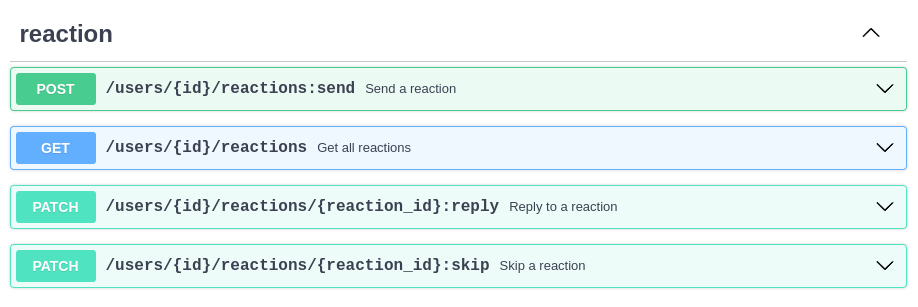
\includegraphics[width=1\linewidth]{swagger_reactions.png}
    \caption{Скриншот из Swagger UI с документацией API сервиса reactions}
    \label{swagger_reactions}
\end{figure}

\begin{figure}[h]
    \centering
    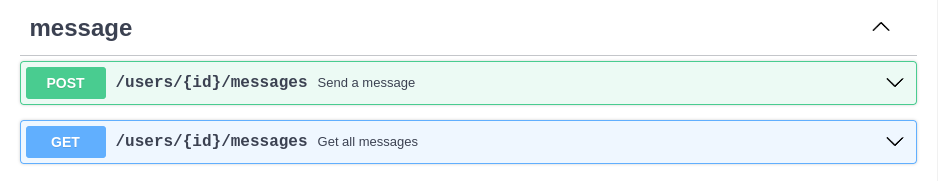
\includegraphics[width=1\linewidth]{swagger_messenger.png}
    \caption{Скриншот из Swagger UI с документацией API сервиса messenger}
    \label{swagger_messenger}
\end{figure}

\textbf{Reactions:} 
Сервис reactions был разработан на базе Spring Boot 3 и Java 21 с подключением к базе данных PostgreSQL. Данный микросервис интегрируется с сервисами profiles и messenger через gRPC, что обеспечивает эффективное взаимодействие и передачу данных между компонентами системы.

\textbf{Процесс развертывания:}
Я также разработал и реализовал процесс развертывания приложения, начиная от создания pull request до загрузки контейнеров в реестр Docker. Пример выполнения процесса можно увидеть на рис. \ref{ci_pipeline}. 

\begin{figure}[h]
    \centering
    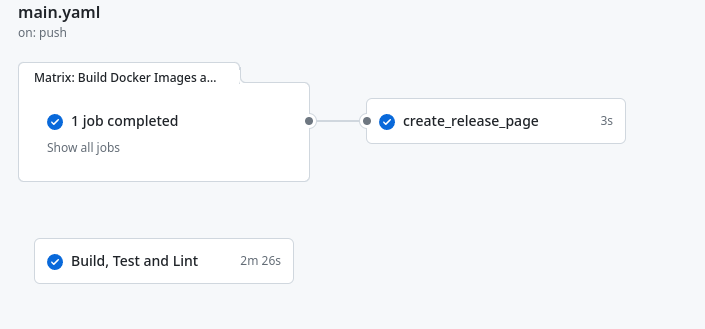
\includegraphics[width=1\linewidth]{ci_pipeline.png}
    \caption{Скриншот из Github Actions с процессом CI/CD}
    \label{ci_pipeline}
\end{figure}

\textbf{Развертывание окружений:}
В рамках этой работы были развернуты два окружения: тестовое и продуктовое.

\begin{itemize}
    \item \textbf{Тестовое окружение:} Развернуто на виртуальной машине в cloud.ru (бывший sbercloud) с использованием Minikube. Это позволило нам проводить интеграционные и нагрузочные тестирования в условиях, максимально приближенных к боевым.
    \item \textbf{Продуктовое окружение:} Развернуто на полноценном кластере Managed Kubernetes от cloud.ru с 16 vCPU и 32 ГБ RAM с использованием Helm charts. В данном окружении были развернуты все компоненты бэкенда, Kubernetes Dashboard и Loki-stack для мониторинга. Пример состояния кластера можно увидеть на рис. \ref{kubernetes_dashboard}.
\end{itemize}

\textbf{Мониторинг и дашборды:}
Для мониторинга состояния системы и визуализации метрик я развернул Grafana и настроил дашборды, которые предоставляют графики и показатели производительности. Это включает метрики состояния микросервисов, использования ресурсов и задержек запросов, что позволяет оперативно отслеживать и устранять возможные проблемы в работе системы. Пример дашборда для сервиса messenger представлен на рис. \ref{grafana_dasboard}.

\begin{figure}[h!]
    \centering
    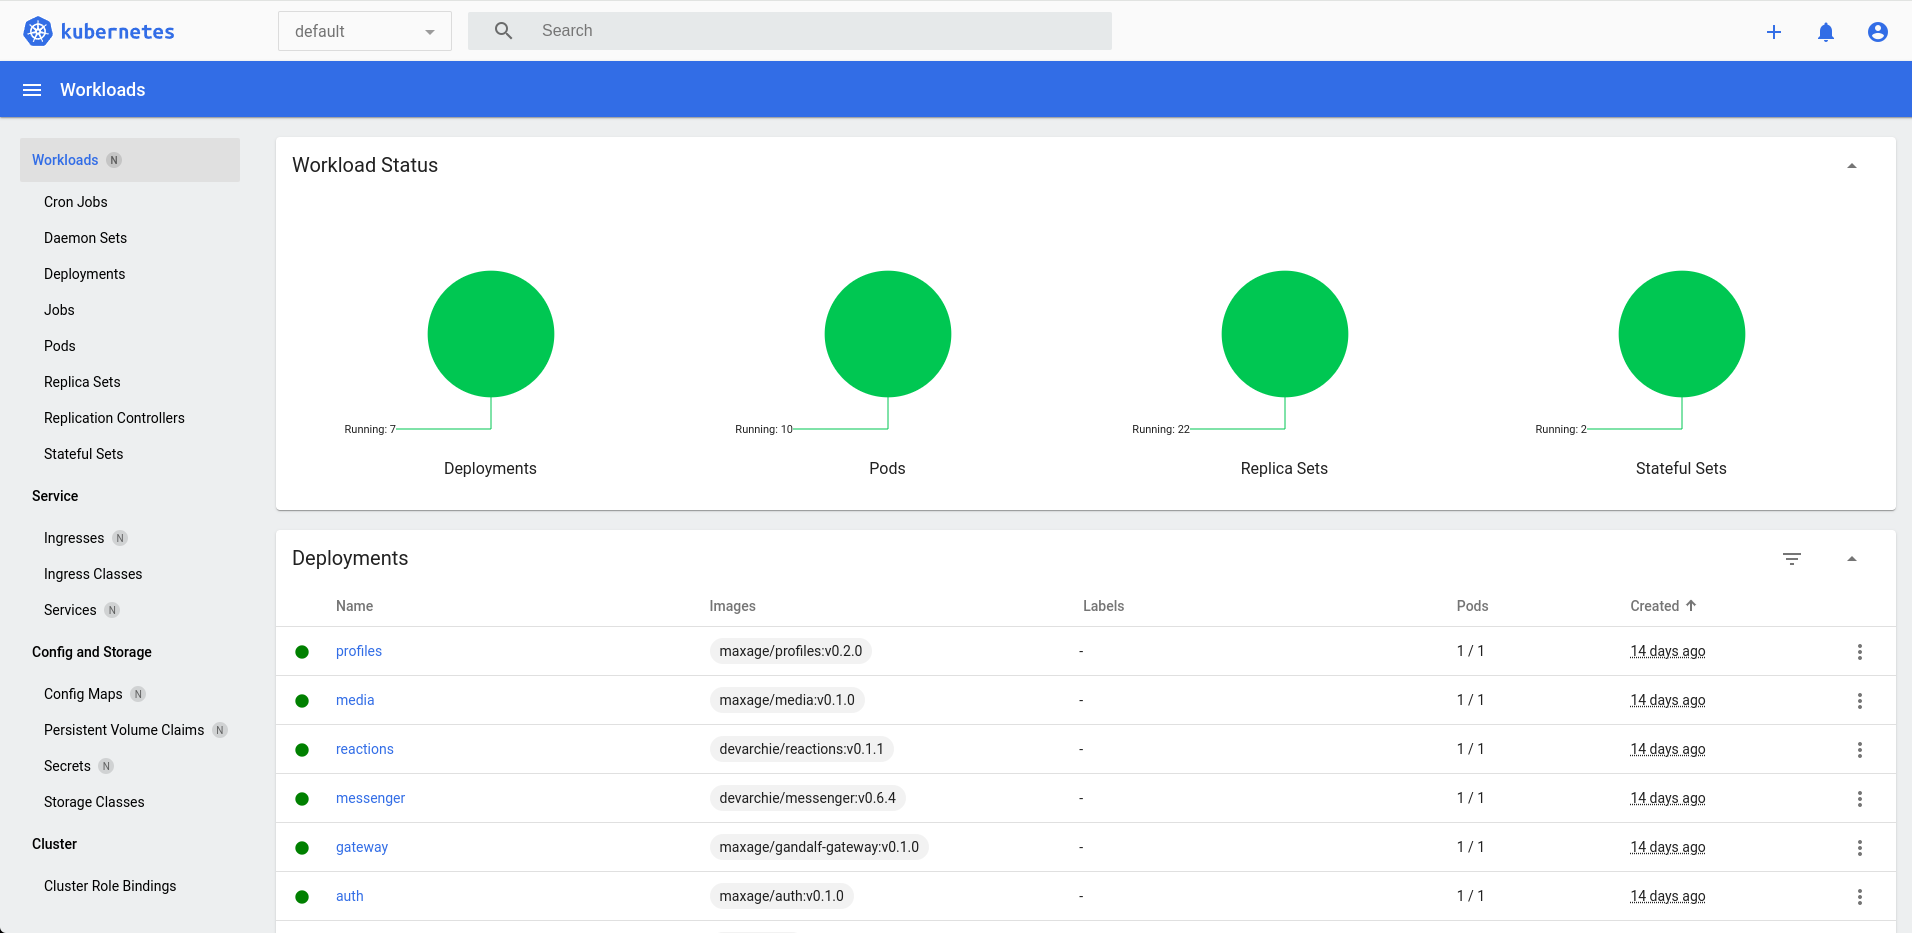
\includegraphics[width=1\linewidth]{kubernetes_dasboard.png}
    \caption{Скриншот Kubernetes Dashboard с состоянием кластера}
    \label{kubernetes_dashboard}
\end{figure}

\begin{figure}[h!]
    \centering
    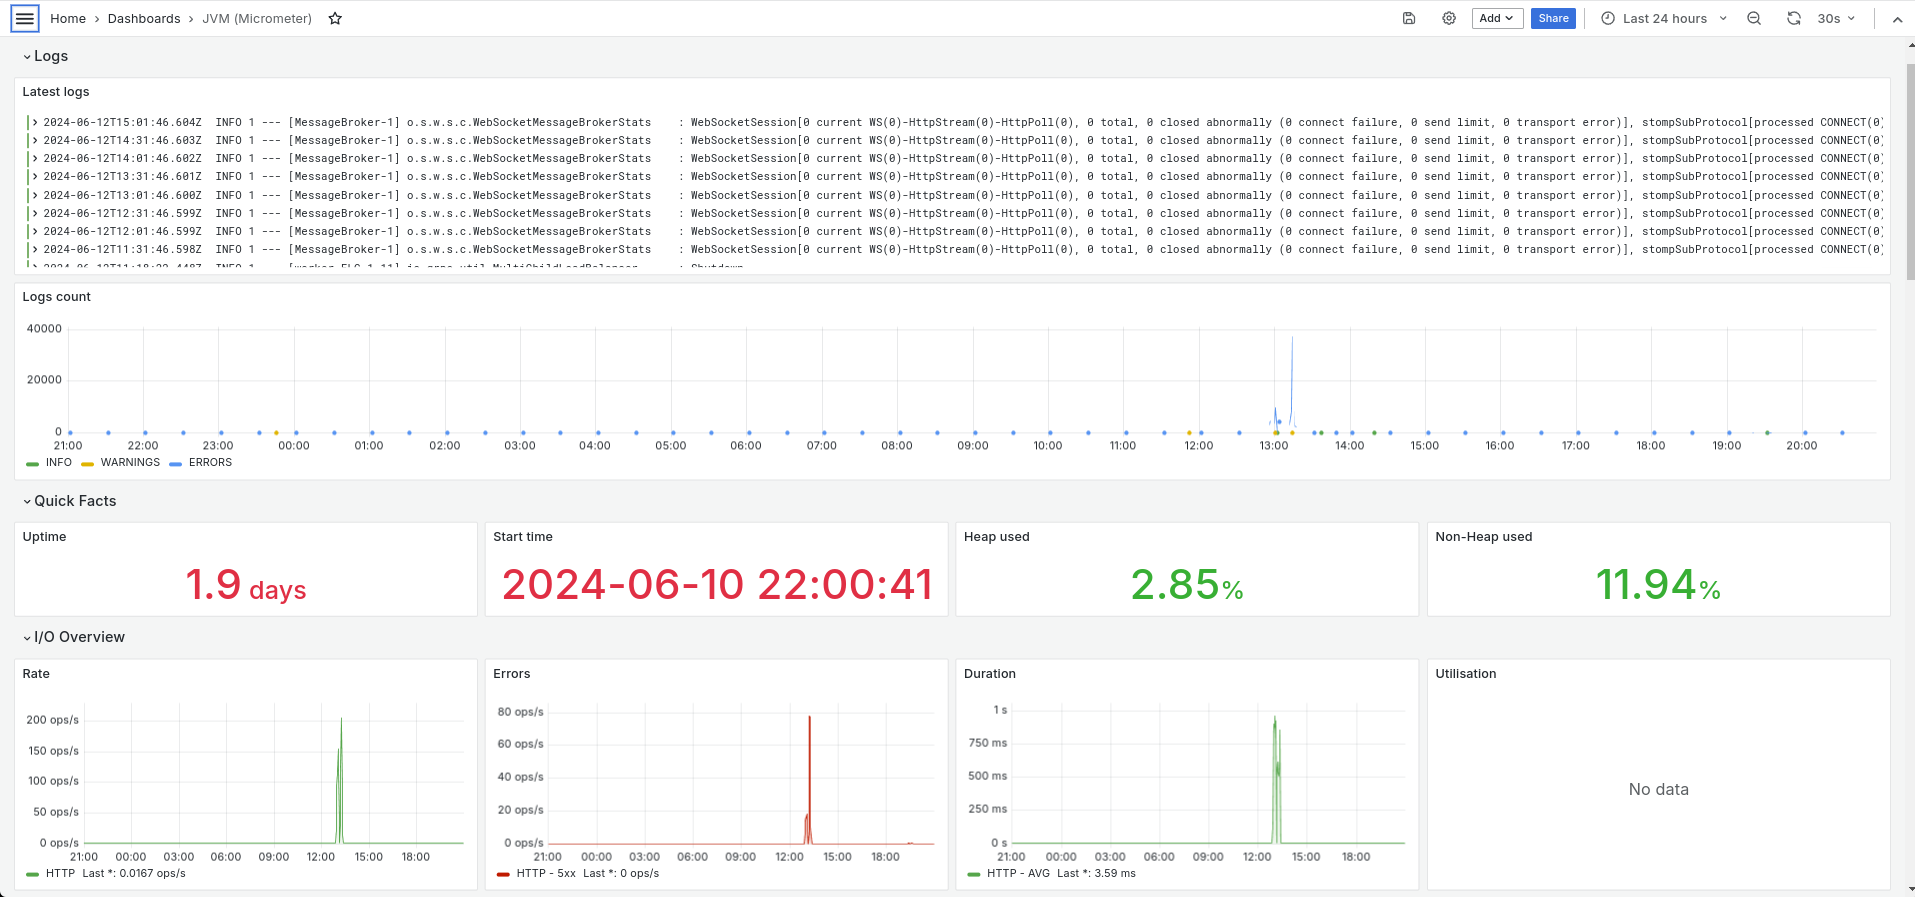
\includegraphics[width=1\linewidth]{grafana_dashboard.png}
    \caption{Скриншот с дашбордом Grafana для мониторинга метрик на примере сервиса messenger}
    \label{grafana_dasboard}
\end{figure}

Таким образом, мой личный вклад в проект включал разработку и реализацию ключевых микросервисов, настройку процессов CI/CD, развертывание и мониторинг тестовых и продуктовых окружений, что в совокупности обеспечило стабильную и производительную работу приложения.



% \newpage

% \begin{thebibliography}{0}
%     \bibitem{jpa Baeldung}\hypertarget{jpa baeldung}{}
%     \href{https://www.baeldung.com/jpa-entities}
%     {balasubramaniam v\@. defining jpa entities| baeldung. --- 2021.}


%     \bibitem{docker Baeldung}\hypertarget{docker baeldung}{}
%     \href{https://www.baeldung.com/ops/docker-compose}
%     {Ligios A\@. Introduction to Docker Compose.}

%     \bibitem{kafka}\hypertarget{kafka}{}
%     \href{https://www.baeldung.com/spring-kafka}
%     {Baeldung. Intro to Apache Kafka with Spring --- 2023}

%     \bibitem{java shild} \hypertarget{shild}
%     {Шилдт Г. Полный справочник по Java\texttrademark Java SE\texttrademark
%         6 Edition. --- 2007.}
% \end{thebibliography}


\end{document}
